\chapter{Overture}\label{chap:intro}
\openepigraph{Écho. Citer ceux du Panthéon et du pont de Neuilly. }{Gustave Flaubert, Dictionnaire des idées reçues}
\openepigraph{Echoes shows the direction that we’re moving in. }{David Gilmour, about the making of ``The Dark Side Of The Moon''}

\vspace{-2.5em}
\marginpar{%
    \footnotesize
    \textbf{Resources:}
    \begin{itemize}
        \item[\faYoutube] \href{https://www.youtube.com/watch?v=lLUcOFwZvyY&t=22s}{Testing The World's Longest Echo}
        \item[\faYoutube] \href{https://www.youtube.com/watch?v=px3oVGXr4mo}{SKUNK BEAR : What Does Sound Look Like?}
        \item[\faYoutube] \href{https://www.youtube.com/watch?v=ZwgovJSQ5UM}{ARTE : La Magie Du Son}
        \item[\faYoutube] \href{https://www.youtube.com/watch?v=uH0aihGWB8U&t=631s}{Daniel Kish: How I use sonar to navigate the world}
    \end{itemize}

}


\def\MyText{\textsc{Echoooes}}
\newcommand\mytext[2][black]{\scalebox{#2}{\textcolor{#1}{\MyText}}}

\newthought{In a nutshell,} this \PhD/ thesis is about acoustic
\stackinset{c}{4ex}{c}{ 1.4ex}{\mytext[black!70]{.8}}{%
\stackinset{c}{2ex}{c}{ 3.2ex}{\mytext[black!25]{.7}}{%
\stackinset{c}{3ex}{c}{-1.3ex}{\mytext[black!35]{.9}}{%
\mytext{1}%
}}}.
\\We live immersed in a complex acoustical world, where every concrete thing can sound, resound and echo.
For humans it is difficult to imaging sound, its constituents and its generation.
In fact, it is processed by our auditory systems and brain so efficiently that our attention is detached from the physical laws governing it.
Therefore, when listening to something, we typically focus directly on its \textit{semantic content}.
Evolution lead us to conduct this process without any efforts, despite the presence of huge level of background noise, for instance in a during a concert.
This outstanding capability is not limited to humans and is common to all the creatures we are sharing the physical world with.

% When we listen to music, we focus on the melody in the music; when listen to speech, we focus on the words;
% \\However not only \textit{semantic information} about the source is carried by the sound.
% There are many other types of information that we retrieve and infer from it, such as \textit{temporal} and \textit{spatial} information.
% For instance, we are able to localize its source:
% if someone is calling us, we unconsciously know towards where to turn.
% We can guess if an noisy motorbike is approaching or moving away.
% Another striking example, which involves simple math, is estimating of how far the storm is, simply counting the time between a view a lightning a listening to thunder.
% We can even guess the size and the type of the room we are currently sitting in.

\mynewline
Nonetheless, we process \textit{all} the information of the complex \textit{acoustic scene} we are immersed into.
In addition to the semantic content, sound conveys also \textit{temporal} and \textit{spatial} information.
For instance, the tickling of a metronome or clock provide units of time\marginpar{
    \footnotesize\itshape
    For his experiments, Galileo Galilei was measuring time using the sound of a metronome.
}
And when hearing someone shouting, we unconsciously know where to turn our attention.
Therefore, as for the content, this information is still carried by the sound.
However, this information is determined by how sound \textit{propagates} in the space and not in the source itself.

\mynewline
While reaching the ears, sound propagates in all direction and portion of its energy arrives to us directly, other indirectly after being reflected around.
This process leads to the creation of \textit{echoes} and \textit{reverberation}.
Typical examples are the echoes produced by huge rocky mountains or by huge walls in monumental buildings, such as the Panthéon in Rome or the pont de Neuilly in Paris.
Echoes refers to particular reflected sound which can be hear distinctly, thus, characterized by specific \textit{time of arrival} and \textit{attenuation}.
In smaller environments, echoes are still present, but are typically less perceived as they arrive more quickly and densely.
What is actually perceived here is the so called reverberation, for which large empty rooms or churches are great examples.

\mynewline
Some animals are evolved to ``see'' through echoes.
For instance, the two (of the most) striking examples are bats and whales which use them as navigation and hunting.
By emitting sound patterns and listening their echoes returned form the environmental, these animals scan the surrounding space, identifying and locating objects.
Here the echoes are voluntarily produced and this is referred to as \textit{active echo-location} or (bio) sonar.
As opposed to, in \textit{passive} echo-location the source sound is not emitted, but rather only received.
\marginpar{
    \footnotesize
    \itshape
    This technique is developed instinctively by some blind people as well.
    By tapping their canes or clicking their tongues, they are able for instance to avoid obstacles when walking.
    The French philosopher Denis Diderot in 18th century recorded the this incredible ability, which was labeled as ``echo-location'' only 300 years later by Donald Griffin.
}.
``Locating it'' means estimating its delay with respect to the direct sound.
These delays are then processed as distances n the brain, in the same as our grandparents taught us to localize storm by counting the time between a lightning and its thunder.
That is how bats and whales find preys, see obstacles and orientated in dark caves or in the deep seas.
However, the term ``echo-location'' here could be misleading as it may refer to the only problem of locating objects.
As we will discuss later, the application of echoes goes beyond simple localization.
Therefore, in this thesis, we will change it in favor of \textit{echo estimation}.

\mynewline
Remarkable examples of passive echo estimation in nature are not very known.
Sand scorpions uses the propagation of vibration in sand to follow the movement of other insect in the dark night.
By using their 8 legs as a radar, they perform passive (seismic) echo-location with inevitable consequences for the prey.
This technique is common to spiders who sense to the reverberation in their complex web\sidenote{
    According to some recent studies, spiders appear to offload cognitive tasks to their webs.
    The web may acts then as a complex system processing and filtering the information, which are then returned to their owner.
    \citeonly{sokol2017thoughts}
}.
They are not only able to localize the preys fast, but also identify them, and disambiguate from simple objects move by the wind or malicious visitors.
In this case, instead of emitting sound, evolution taught them to uses complex structures (for scorpions their legs, for spiders webs) in order to feed and survive.

\mynewline
Echoes do not only serve for computing distances or localizing preys.
For instance, they make speech more intelligible, provide music with ``dimensionality''\citeonly{sacks2014musicofilia} and improve our sense of orientation and balancing.
This phenomenon is material of studied in \textit{room acoustics}, \textit{pyschoacoustics} and \textit{sound design}.
In particular, the former study acoustic echoes for designing theatres, auditoriums and meeting rooms, whose actual propose is to listen well.

\mynewline
% To conclude with, this thesis focuses on how to estimate passively acoustic echoes and how to used them to achieve better audio analysis.
% This investigation is conducted in the context of indoor audio signal processing.
The problems addressed in this thesis are indicated in the thesis title: \textit{Echo-aware signal processing for audio scene analysis}.
There are three parts in the sentence that deserve an explanation: \textit{echo-aware}, \textit{signal processing} and \textit{audio scene analysis}.
In turn, we will elaborate first the last two as they contextualize the this thesis, immediately after, we will explain why and how echoes helps.

% \mynewline
% One may ask, what does it mean, to estimate echoes and use them?
% Therefore with echo estimation we will refer to the estimation of them both.
% Even there are less clear example in nature to explain it, passive echo location is used by our mind instinctively in order to process the acoustic scene.
% Therefore, in the context of computer science, it is natural to ask ourself how we can build machine that can listen as we do?
% How is it implemented? it will be outlined in the next section.

\section{Audio Signal Processing}\label{sec:intro:processing}
% In order to process sounds, machines and computer use algorithmic tools which fall in the research field of \textit{audio signal processing}.
\textit{Signal processing} is the process of analyzing and modifying a \textit{signals}, which are mathematical representation of quantities carrying information about a phenomenon.
Then, \textit{audio signal processing} represents sound, such as music or speech, as signals
\marginpar{
    \footnotesize
    \textit{Audio is a more technical term, referring to sound coming from a recording, transmission or electronic device.
    Acoustic, instead refer to the physical aspect of the sound.
    \\In this thesis, the two terms are used indistinctly.}
} and it involves applying various mathematical and algorithmic techniques to them.
There are multiple reasons to do this, such as produce new signals with higher quality or and retrieve high-level information that the signal carries.
To this end, complex systems are built which can be represented as collection of simpler subsystems, with well-defined tasks, interacting with each other.
In (audio) signal processing, these subsystems roughly fall into four categories: \textit{representation}, \textit{enhancement}, \textit{estimation}, and \textit{adaptive processing}.
Many related problems can be then decomposed into blocks one or more of the following steps.

\newthought{Representation}.
    The signal can be represented in many different way, so that the \textit{information} they contain becomes more suitable for certain tasks.
    It is generally implemented through change of \textit{domain} or \textit{feature}.
    In case of audio, the most famous representation is the Fourier basis, which change the signal domain from from time to frequencies.

\newthought{Enhancement}.
    Measurement are affected by \textit{noise} which corrupt and hide the relevant information.
    Therefore, signal enhancement, namely, removing noise, is typically a necessary step.
    Example of enhancement are removing background noise from a mobile phone recording or isolate instrument tracks from in a song, \etc/.

\newthought{Estimation}.
    Often we wish to estimate some key properties of the target signal which may be used as inputs to a different algorithm.
    For instance, the position of a speaker in a recording, the time of arrival of a echo, the frequency of a sound with respect to the background noise.

\newthought{Adaptive processing}.
    It deals with adaptive algorithms which are controlled by variable parameters resulting on previous estimation blocks.
    They usually rely on online optimization of objective function designed to meet certain requirements.
    Example of these algorithmic are present in noise cancelling headphones or echo cancellation modules implemented in video conference call systems.

\section{Audio Scene Analysis}\label{sec:intro:scene}
Pay attention to what are you listening now:
there might be music, someone talking to you, footsteps echoing in a other room, background noise due to cars, heating system, maybe rain or wind, the sound of your own movement and many other.
Everything you are hearing now as well as its location in space, is what is called the \textit{audio scene}\sidenote{
    The more correct terminology for it is \textit{auditory scene}, which relates to the human perception.
    It was coined by psychologist Albert Bregman in~\citeonly{bregman1990auditory}.
    However we will use this terminology since we extend this concept to audio signal processing and as it is commonly accepted in the literature.
}.
Therefore, the \textit{audio scene analysis} is trivially the analysis of it\marginpar{
    \footnotesize\itshape
    From the anacient greek, \emph{analysis} literally means dismantling into constituent elements.
    It allows then to reach information otherwise obfuscated by the big picture.
    It is opposed to \emph{synthesis} which instead combines parts into a whole.
}.
More specifically, the extraction and organization of all the information contained by the sound associated to an audio scene.

\mynewline
% This scene is not only listened by you, but it may be listened (or ever recorded) by your mobilephone, your laptop or your smart home device.
In the context of audio signal processing, this process involves using algorithmic and mathematical tools aiming at retrieve and organize such information.
After recording the audio scene with microphones, complex systems, as described above, are used to access the information.
Accessing different types of information at different levels of complexity lead to the definition of different \textit{problems}.
These problems focuses on well defined tasks in the general audio scene analysis and some of them are referred to with established names.
\cref{tab:processing:problems} lists some selected audio scene analysis problems that will be considered later in this thesis.

\begin{table}[!h]

    \begin{fullwidth}
    \centering
    \small

    \begin{tabular}{p{0.33\linewidth} p{0.66\linewidth}}
    \toprule
    Problems & \textit{From the recordings, can we...} \\
    \midrule
    Audio Source Separation   & ... estimate the audio signal of sound sources?\\

    Audio Source Enhancement   & ... estimate the audio signal of a target sound source?\\

    Sound Source Localization & ... estimate the positions of sounds sources? \\

    Microphone Calibration    & ... positions and properties of the microphones?? \\

    Room Geometry Estimation  & ... estimate the shape of the room? \\

    Acoustic Echo Estimation  & ... estimate the echoes' properties? \\

    Acoustic measurement      & ... estimate physical properties related to sound propagation?\\

    \hline
    Source Identification     & ... estimated the type of source signal?\\

    Speech Diarization        & ... who is speaking and when ? \\

    Source Counting           & ... count the number of speaker s? \\

    Automatic Speech Recordings & ... the content of the speech ? \\

    \bottomrule
\end{tabular}
    \caption{List of selected audio scene analysis problems. The one above the line are considered in this thesis.}
    \label{tab:processing:problems}

    \end{fullwidth}

\end{table}

\mynewline
Without going to philosophically, it is possible to re-cast these problems to some (simple) human interrogations that :
\begin{itemize}
    \item  \textit{What?} Answered by Audio Source Separation and Enhancement, Speech2Text and Source Identification, by operating on the semantic content of the source signals.
    \item  \textit{Where?} Answered by Sound Source Localization, Microphone Calibration and Room Geometry Estimation, by elaborating the spatial information of the sound propagation.
    \item  \textit{When?} Answered by Speech Diarization, by leveraging on the sound temporal information.
\end{itemize}

\mynewline\openepigraph{Everything is connected}{Douglas Adams, \textit{Dirk Gently's Holistic Detective Agency}}
Our brain and auditory system is able to solve this problems instantly and effortlessly, such that they may sounds trivial tasks.
However, they hide many difficult challenges when it comes to design efficient and robust algorithms.
Moreover, most of the all these problems may exhibits strong inter-connections, and the solution of one depends on the solution of another.
For instant, by knowing knowing when someone is speaking and its location in the room, sound source separation can be achieved more easily.
It should not surprise and have strong parallelism with the our every day experience.

\mynewline
And this is why echoes may help audio signal processing.


\section{Echo-aware approach}
As proven by natural behaviors, acoustic echoes are essential for human and animals for analyzing the audio scene:
As repetition of a sound, they convey information about that sound.
As characterized by temporal instant and attenuation related to distances, they convey spatial information about the audio scene.
As modified by the frequency description of the object which generate them, they convey acoustic information about the such object.
\\This observation motivated many researcher to include echoes in signal processing applications, not only limited to audio\sidenote{
    The idea of integrating reflection in models studied also in other field of engineering.
    In telecomunication and in networking for instance, where this phenomena are referred to as \textit{multipath propagation}.
}.
However it was not always the case.
In order to derive efficient algorithms, many audio scene analysis methods make strong assumptions of the sound propagation.
One of the most common one is the so-called anechoic or free-field scenario, namely, assuming neither echoes or reverberation are present in the audio scene.
Even if this assumption can be reasonable in some scenario, it is then easy to understand the limitations when dealing with real world recordings.
In some cases, they are considered as source of noise and interference and then to be removed.


\mynewline
Instead, some researchers proposed to explicitly include acoustic echoes in their models, which we will refer to as \textit{echo-aware methods}.
One of the earliest examples in this direction are the work of Flanagan et al\citeonly{flanagan1993spatially, jan1995matched, jan1996sound} for in source enhancement.
However, only recently these methods have regained interested for audio processing as manifested by the European project SCENIC~\citeonly{Annibale2011scenic} and the UK research \href{http://www.s3a-spatialaudio.org/}{S$^3$A project}.
In some recent studies, echoes are used boosts performances of typical audio scene analysis problems, \eg/, speech enhancement \citeonly{Dockmanic2015raking, Kowalczyk2019raking}, sound source localization \citeonly{ribeiro2010turning}, and separation \citeonly{scheibler2017separake, leglaive2016multichannel, Remaggi2019modeling}, and room geometry estimation from sound \citeonly{remaggi2016acoustic, dokmanic2013acoustic, crocco2017uncalibrated},

\mynewline
All this methods show the importance and the benefits of modeling acoustic reflection, however prior to all them is the \AERdef/.
This step, which is typically given for granted in the above application, is extremely challenging as shown throughout this entire work.


% \newthought{Audio Signal Processing}
% \begin{itemize}
    %     \item Motivation
    %     \item Definitions, Function, Characteristics
%     \item Current challenges
% \end{itemize}

% \newthought{Inverse Problem}
% Starting with the effects to discover the causes has concerned physicists for centuries.

% While in many ways, mixtures are not different to any other audio signal, two research questions stand out prominently: • Can we obtain the sources sj from the mixture x? • Can we find the number of sources J from x? These two questions are addressed in the scientific fields of sound
% source separation and source count estimation


% Inverse problems appear when we want to see or examine something that we cannot access directly. What we have is an indirect measurement that contains hidden information.

% An inverse problem is always a counterpart of a direct problem, as shown in the schematic diagram below. The direct problem is going from object to data, and the inverse problem is about finding the object back from the data.

% The assumed few thousand taps. This model was very popular in the early stages of research [48]–[55]. Recently, interest has revived with sparse penalties which account for prior knowledge about the physical properties of AIRs, namely the facts that power concentrates in the direct path and the first early echoes [56]– [60] and that the time envelope decays exponentially [61], but these penalties have not yet been used in a BSS context.


% \section{Audio Inverse Problems}\label{sec:processing:inverse}
% \cite{kitic2015cosparse}
% \openepigraph{Their generality is of such a wide scope that onemayeven argue that solving inverse problems is what signal processing is all about}{Srdan Kiti\'c, \textit{Cosparse regularization of physics-driven inverse problems}}
% \openepigraph{everything is an optimization problem}{\citeonly{watson2001nonlinear}}
% \marginpar{
%     \footnotesize
%     One can see the paralelism with the engineering concepts: analysis and sythesis.
% }
% In~\cref{sec:intro:problem} we have informally defined \textit{inverse problems}, with an emphasis on inverse problems in signal processing.
% An inverse problem is a type of a mathematical problem where we start with the observations and we want to estimate model parameters that produced them.
% \\Inverse problems pervades all the field of science and engineering:
% source localization~\cite{},
% image processing~\cite{},
% acoustic imaging and tomography~\cite{},
% \marginpar{
%     \footnotesize
%     A historical example are the calculation of the Earth circunference by Eratosthenes in III century b.c.\\
%     and the calculations of Adams and Le Verrier which led to the discovery of Neptune from the perturbed trajectory of Uranus.
% }

% A inverse problems is defined as the counterpart of a \textit{forward}\sidenote{often referred to as \textit{direct}} problem.
% Without falling in and deep mathematical formalism and taxonomies which can be found in \citeonly{bal2012introduction},
% we will simply consider the following informal definition:
% \begin{center}
%     \textit{\emph{Forward problem} starts from known input, while \emph{inverse problem} starts from known output~\cite{santamarina2005discrete}.}
% \end{center}
% Both these problems focus on an operation relating maps objects of interest, called \textit{parameters} or \textit{variables},
% to information collected about these objects, called \textit{measurements}, \textit{data} or \textit{observation}.

% For instance, in our context, the direct problem may be the estimation of the \RIR/(s) starting from the known room parameters,
% and, the related inverse problem would be the estimation of such room properties from the observation of the \RIR/(s).

% Formally, a forward problem is defined through a mathematical model, described by a \textit{operation} $\scrM(\cdot)$
% mapping \textit{parameters} $x \in \scrX$ to the \textit{observation} (or measurement) $y \in \scrY$:
% \begin{equation}\label{eq:processing:model}
%     y = \scrM(x)
%     .
% \end{equation}
% Then, the inverse problem defines a method $\kinv{\scrM}$ that ``reverts'' $\scrM$ in order to recover (estimate) $x$ form the observation of $y$.
% % The operator $\scrM$ describes our best effort to construct a \textit{model} for the available data $y$.
% % The choice of $\scrX$ describes our best effort to characterize the space where we believe the parameters belong.

% As discussed in~\cite{bal2012introduction}, \textit{solving} the inverse problem consists in finding point(s) $x \in \scrX$ from (knowledge of) data $y \in \scrY$
% such that~\cref{eq:processing:model} or an approximation of~\cref{eq:processing:model} holds.
% Under this light, the operator $\scrM$ ant the choice of $\scrX$ describes our best effort to construct a \textit{model} for the data $y$ and
% the space where the parameters $x$ belong, respectively.
% \marginpar{
%     \footnotesize
%     one can already see the paralelism the the definition of the mixing process defined in~\cref{sec:intro:problem}
% }

% \textsc{For instance, in Case of} \textit{linear} inverse problem, and for $\scrY$ and $\scrX$ being vector spaces of dimensions $M$ and $N$ respectively,
% then the forward map can be written as a linear system:
% \begin{equation}\label{eq:processing:linear_forward}
%     \bfy = \bfM \bfx
% \end{equation}
% where $\bfM$ being a matrix, namely the operator $\scrM$ becomes a matrix multiplication by $M$.
% It follows that the inverse map associated to~\cref{eq:processing:linear_forward} is the application of the inverse matrix $\kinv{M}$.
% % While solving a direct problem the an operator needs to be found, in solving the inverse one either the operator is known and needs
% % to be $reverts$t

% Typically, forward problems are considered somehow the ``easier''.
% In fact, even in the observation model $\scrM$ is known perfectly, it is not always possible to find its counterpart.
% This because of
% \begin{itemize}
%     \item presence of \textit{noise} in the measurement which are not always additive and statistically independent \wrt/ $x$.
%     \item the problem is \textit{well-posed} and \textit{well-conditioned}, namely $\scrM$ needs be injective and stable.
%     In other words, some information is recoverable, other is completely lost, other highly sensible to noise
%     \sidenote{
%         \textbf{injective} ensure the uniqueness of the solution, while \textbf{stability}
%         ensure a continuity on the data.
%         These are known as the Hadamard's \textit{solvability conditions}.
%     }.
% \end{itemize}

% As we could images, many interesting and fundamental inverse problem are
% \textit{ill-posed} or \textit{ill-conditioned} in general, even in the following ``simple'' ones~\cite{kitic2015cosparse}:
% The solution to the deconvolution problem, where the direct inversion of the transfer function results in instabilities
% at high frequency; and the solution a linear system $\bfy = \bfM \bfx$ where $\bfM$ is invertible
% may lead to erroneous results and numerical instabilities.

% Therefore, sometimes ones have to settle for restring the set of solution $\scrC \subset \scrX$,
% where $\scrM$ is stable and injective\sidenote{This framework was originally proposed by Tikhonov.}.
% Promoting solution $x \in \scrC$ is can be achieved through \textit{model priors}, namely prior knowledge about solution, which can
% be classified in the following methodologies:
% the usage of \textit{geometric constraints} that deterministically define the solutions; the imposition of \textit{penalization}
% which ``promotes'' solution of a certain shape (\eg/ \textit{sparse}
% \sidenote{\textbf{sparsity} is a fundamental concept of this thesis, better discussed in~\cref{pt:estimation}
% } or \textit{smoothness});
% and casting the problem in a \textit{bayesian framework} which versatilely incorporate prior and posterior density function describing the data.

% Let us give two example of practical systems that will be recurrent thought out the entire thesis.

% \subsection{Selected Audio Inverse Problems}
% Here follow some famous problems in the field of audio signal processing with application to speech, music and environmental audio.
% Given the mixing process defined in~\cref{sec:processing:model},

% % \begin{description}
% %     \item[sound source separation and enhancements] as the problem of retrieving a (set of) source signal from a mixture.
% %     \item[sound source localization] estimation of source location from the observation of the sound production.
% %     This has sense as long as the impulse response convey space properties.
% %     \item[microphones calibration] estimation of the microphone placement.
% %     \item[\RIR/ estimation] estimation of the filters.
% %     Blind Channel Estimation or System Identification.
% %     \item[Acoustic Echoes Estimation] estimation of the filters
% %     \item[dereverberation] estimation of the filters
% %     \item[room geometry estimation] estimation of the room
% %     \item[automatich speech recognition]
% % \end{description}



%
% \newthought{Depending on the scenario}, all these problems exhibits strong inter-connections,
% namely the solution of one may be (dependent on) the solution of another.
% Therefore, exploiting expertise and knowledge,
% interconnect and hierarchical approaches may be built\sidenote{Machine Learing allows now for end2end approaches}:
% for instance, many spatial filtering techniques used for \SE/ rely on \SSL/ blocks;
% and in order to achieves \RooGE/, \AER/ must be done.



\section{Thesis Outline and Main Contributions}\openepigraph{Sometimes a scream is better than a thesis.}{Ralph Waldo Emerson}
The goal of this thesis is to improve the current state-of-the-art in indoor audio signal processing along two axes:
\begin{enumerate}
    \item Provide new methodologies and data to process acoustic echoes and surpassing the limits of current approaches.
    \item Extend previous classical methods for audio scene analysis by incorporating the knowledge of these elements of the sound propagation.
\end{enumerate}

\mynewline
These two claims are elaborated in the two main part of the thesis which follow after an introductory one, as summarized below.
However the parts are largely interconnected, as show in the~\cref{fig:intro:thesis_mindmap}:

\begin{figure}[t]
    \begin{sidecaption}[Thesis Organization]{%
        Schematic rganization of the thesis, dependecies between chapters linked to author contributions.
    }[fig:intro:thesis_mindmap]
    \centering
    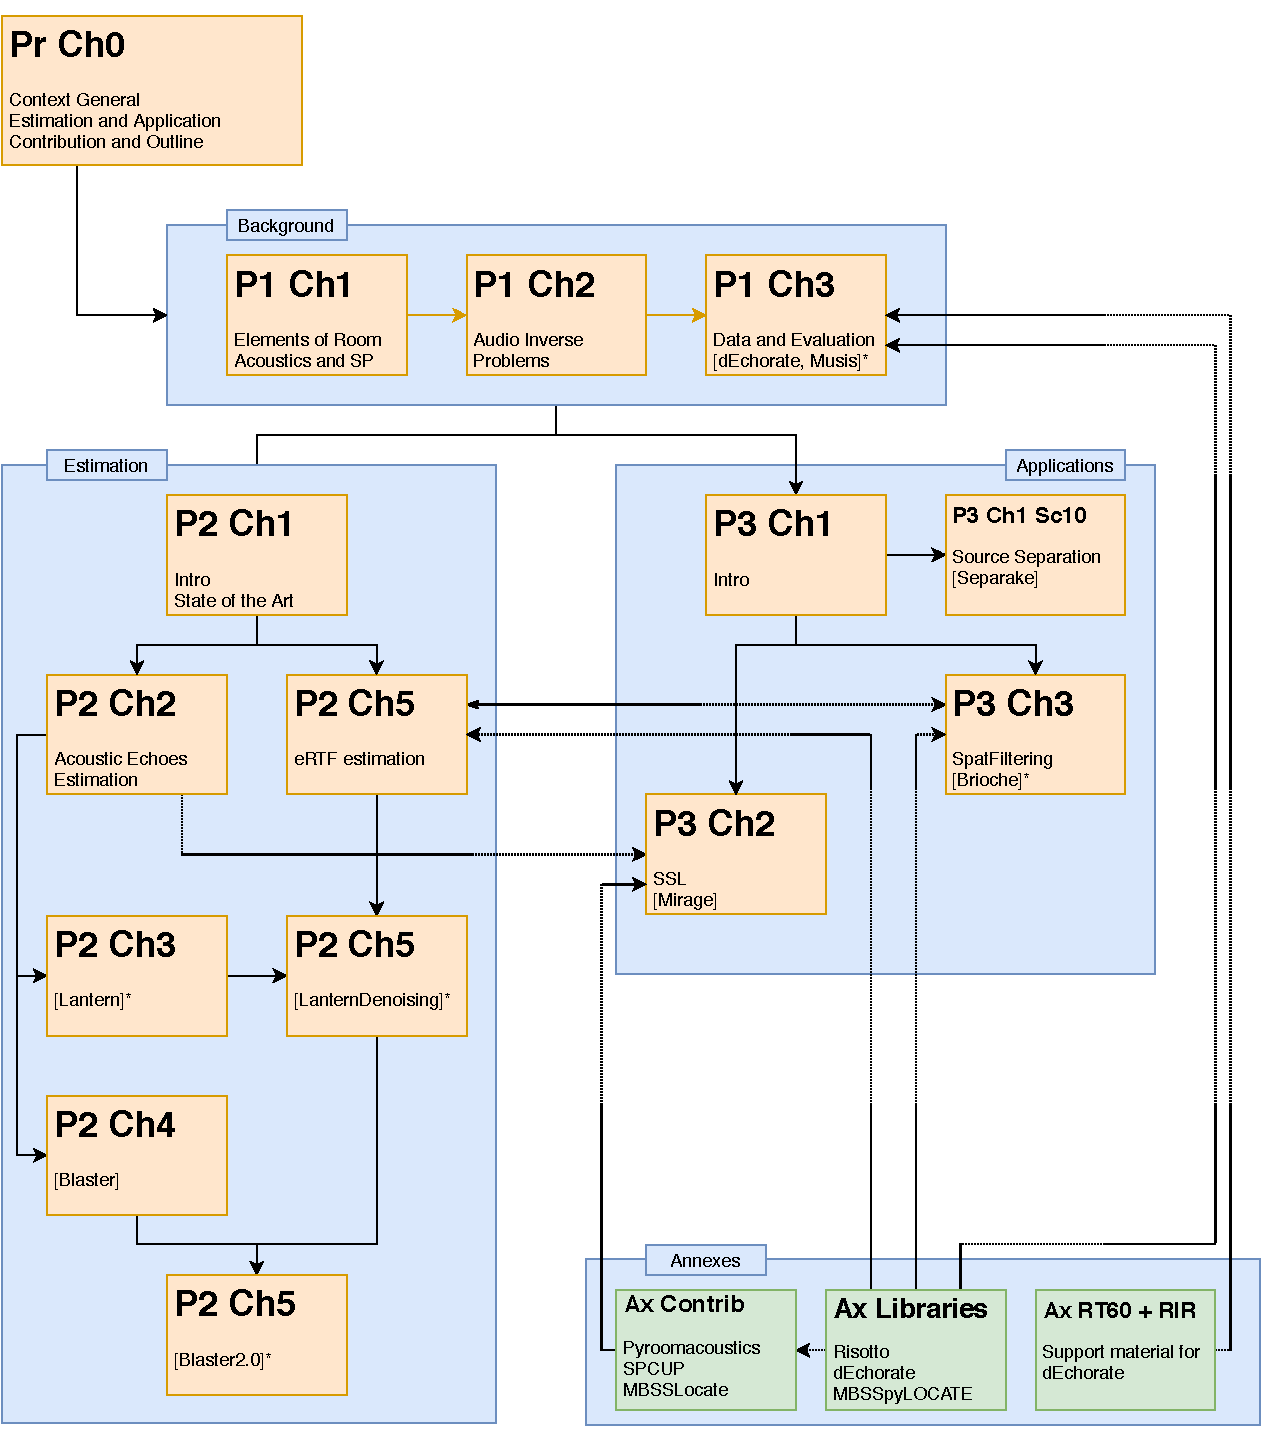
\includegraphics[width=\linewidth]{intro/thesis_mindmap.pdf}
    \end{sidecaption}
\end{figure}


\newthoughtpar{Room Acoustic meets Signal Processing}
\begin{description}
    \item[\cref{ch:acoustics}]\synopsisChAcoustics
    \item[\cref{ch:processing}]\synopsisChProcessing
\end{description}

\newthoughtpar{Acoustic Echoes Estimation}
\begin{description}
    \item[\cref{ch:estimation}]\synopsisChEstimation
    \item[\cref{ch:lantern}]\synopsisChLantern
    \item[\cref{ch:blaster}]\synopsisChBlaster
\end{description}


\newthoughtpar{Echo-aware Audio Scene Analysis}
\begin{description}
\item[\cref{ch:application}]\synopsisChApplication
\item[\cref{ch:separake}]\synopsisChSeparake
\item[\cref{ch:mirage}]\synopsisChMirage
\item[\cref{ch:brioche}]\synopsisChDecharateApp
\end{description}

\newthought{Finally,} the dissertation concludes with Chapter 13, which summarizes the contributions and raises several additional research questions.


\section{List of Contribution}
This dissertation draws heavily on the earlier work and writing in the following papers, written jointly with several collaborators:

\begin{itemize}
    \item \fullcite{di2021dechorate}
    \item \fullcite{di2020blaster}
    \item \fullcite{di2019mirage}
    \item \fullcite{deleforge2019audio}
    \item \fullcite{lebarbenchon2018evaluation}
    \item \fullcite{scheibler2018separake}
\end{itemize}


\section{Don't Panic!}
The reader will have already noticed that a large margin is left free on each page of the manuscript.
We will use it to insert personal comments, historical notes, additional insights as well as figures and tables to complete the each chapter subject.
This graphic template is inspired by the work of \citeauthor{tufte1983visual}\citeonly{tufte1983visual}\sidenote{
    Information on the template is described in the colophon of the thesis.}
.
We emphasize that the presence of the clickable link by the \ExternalLink logo as well as code library which are written in typewrite font, \eg/ \library{dEchorate}.
\\A list of design choice follows:

\subsection{Quick vademecum} for the readers:
\begin{itemize}
    \item Bibliographic references are denoted as \citeonly{kuttruff2016room}.
    \item Figures, Tables and other floating objects as well as equations are numbered within the chapter number.
    \item Equations are referred as~\cref{eq:acoustics:green_definition}
    \item \ExternalLink denotes clickable external link
    \item \textcolor{myorange}{orange} is used for clickable internal link, such as~\cref{sec:intro:processing} and acronyms \acs{FFT}.
    \item \textcolor{mygray}{grey} is used for clickable internal link, such as \href{www.diegodicarlo.com}{my website\ExternalLink}
    \item Reference sidenotes on the margin are used as footnotes, providing additional insights.
    \item Italic sidenotes and figures without proper reference number on the margin are meant to provide optional information and can be read in a second moment.
    \item \textcolor{black!30}{\scriptsize\raisebox{1pt}{$\blacktriangleright$}} should capture reader attention towards the important points.
    \item \textcolor{black!30}{\scriptsize\raisebox{1pt}{$\rightleftarrows$}} indicate the presence of definition by dichotomy.
    \item The end of the chapter is shown with a logo signature.
\end{itemize}

\subsection{The golden ratio of the thesis}
This thesis has been written following personal stylistic rules:
\begin{itemize}
    \item At most 3 level of sub-headings: section, subsection and Tufte's \textit{new-thought}.
    \item The usage of dichotomies is emphasized.
    \item Each paragraph is introduced briefly at the end of the previous one.
    \item no indentation, but well separated text blocks.
\end{itemize}